\section{Digitale Transformation im Mittelstand}

\newacronym{erp}{ERP}{Enterprise-Resource-Planning}
\newacronym{iot}{IoT}{Internet of Things}

\newglossaryentry{cloud}{%
    name=Cloud Computing,
    description={Bereitstellung von IT-Ressourcen wie Rechenleistung, Speicher und Software über das Internet}
}

Der digitale Wandel betrifft nicht nur Großkonzerne, sondern zunehmend auch kleine und mittlere Unternehmen. 
\acrshort{erp}-Systeme helfen dabei, betriebliche Prozesse zu standardisieren und in Echtzeit abzubilden. 
Sie bilden die Grundlage für datenbasierte Entscheidungen. 
Siehe auch~\gls{cloud}. Siehe dazu auch grundlegende Ausführungen\footcite[vgl.][S.~101]{mustermann2021-chapter}. Vergleiche (Tab.~\ref{tab:tech-vergleich})

\begin{table}[H]
    \centering
    \small
    \begin{tabular}{lccc}
        \toprule
                        & \textbf{ERP-System} & \textbf{IoT-Lösung} & \textbf{Cloud-Service} \\
        \midrule
        \textbf{ERP-System}   & 1    & 3    & 4    \\
        \textbf{IoT-Lösung}   & 2    & 1    & 3    \\
        \textbf{Cloud-Service}& 4    & 2    & 1    \\
        \bottomrule
    \end{tabular}
    \caption[Vergleich digitaler Technologien]{Vergleich digitaler Technologien im Mittelstand\protect\footnotemark}
    \label{tab:tech-vergleich}
\end{table}
\footnotetext{\cite[Eigene Darstellung nach][]{muster2023-article}.}

Neben der Integration von \acrshort{iot}-Sensoren werden zunehmend Cloud-Dienste genutzt, um Daten flexibel und skalierbar zu speichern. 
Dies ermöglicht neue Geschäftsmodelle, etwa in der vorausschauenden Wartung\footcite[vgl.][S.~60]{muster2023-article}.  

\subsection{Einfluss auf Arbeitsprozesse}

Die Digitalisierung verändert nicht nur die Technik, sondern auch die Organisation der Arbeit. 
Vergleiche hierzu (Abb.~\ref{fig:hund}). 
Neue Kommunikationsformen entstehen und klassische Hierarchien werden zunehmend durch agile Arbeitsmethoden ergänzt. 
Aktuelle Einschätzungen liefert der Branchenreport\footcite{muster2024-online}.  

\begin{figure}[H]
	\centering
	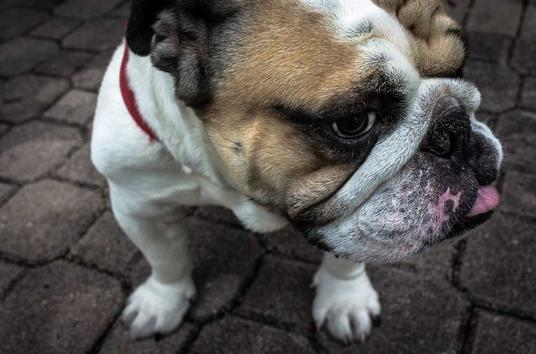
\includegraphics[width=\textwidth]{images/hund.jpg}
	\caption[Hund als Platzhalter]{Ein Hund als Platzhalterabbildung\protect\footnotemark}
	\label{fig:hund}
\end{figure}
\footnotetext{\cite[Veränderte Darstellung nach][7]{mustermann2021-chapter}.}

\subsubsection{Herausforderungen}

Die größten Herausforderungen liegen in der Qualifizierung der Mitarbeitenden sowie im Datenschutz. 
Nur wenn Mitarbeiterinnen und Mitarbeiter ausreichend geschult werden, können digitale Tools effizient genutzt werden. 
Vgl. hierzu auch die Standardwerke\footcite[vgl.][S.~50]{meier2010a} und\footcite[vgl.][S.~75]{meier2010b}.  

\subsubsection{Standards und Regularien}

Unternehmensinterne Richtlinien müssen zudem mit internationalen Normen abgeglichen werden. 
Für spezifische Anforderungen gelten Standards wie\footcite{iso9001-2015-sample}, die Prozesse vereinheitlichen und Qualität sichern.  
